\begin{frame}
	\begin{center}
		
\includegraphics[width=8cm]{ressources/AlphaGoLogo}

	\end{center}
\end{frame}


\begin{frame}{AlphaGo}
	\begin{itemize}
		\item Développé par Google DeepMind
		\item En mars 2016 \textbf{AlphaGo} a battu Lee Sedol, l'un des meilleurs joueurs de Go
		\item Technologies utilisées:
		      \begin{itemize}
			      \item Apprentissage par renforcement
			      \item Réseaux de neurones profonds
			      \item Monte Carlo Tree Search
		      \end{itemize}
	\end{itemize}
\end{frame}



\begin{frame}{AlphaGo}{Composants}
	\begin{columns}[t]
		\begin{column}{.3\textwidth}
			\begin{block}{Rollout policy}
				Politique plus simple que les autres qui permet une simulation rapide du reste de la partie. Elle est amplement utilisée dans la simulation du MCTS.
			\end{block}
		\end{column}
		\begin{column}{.3\textwidth}
			\begin{block}{Policy network}
				Réseau neuronal qui renvoie une distribution de probabilité sur le coups possibles.
			\end{block}
		\end{column}
		\begin{column}{.3\textwidth}
			\begin{block}{Value Network}
				Réseau neuronal chargé de estimer la valuer d'une position, c'est-à-dire, les possibilités de gagner à partir de cette position.
			\end{block}
		\end{column}
	\end{columns}
\end{frame}

\begin{frame}{AlphaGo}{Entraînement des Réseaux neuronales}
	\begin{center}
		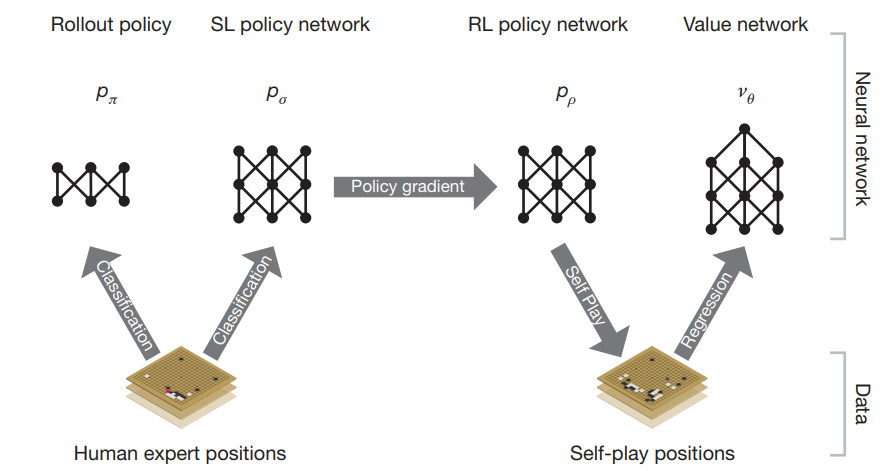
\includegraphics[width=7cm]{ressources/Entrainement}
		\begin{columns}[t]
			\begin{column}{.4\textwidth}
				\begin{block}{Avec un modèle}
					Entrainement d'un réseaux supervisé (SL).
				\end{block}
			\end{column}
			\begin{column}{.4\textwidth}
				\begin{block}{Self-play}
					Apprentisage par renforcement à partir du SL en jouant des parties contre soi-même.
				\end{block}
			\end{column}
		\end{columns}

	\end{center}

\end{frame}


\begin{frame}{AlphaGo}{Apprentissage avec un modèle (SL)}

	\begin{itemize}
		\item Entraînement initial supervisé à partir de parties jouées par des professionnels (30 million de positions différentes).
		\item Le modèle doit prédire, à partir d'un état, le coup qu'un humain aurait fait.
		\item Réseau neuronal de type convolutionnel avec 13 couches.
		\item L’entraînement donne une politique $p_\sigma$, avec $\sigma$ les paramètres (les poids) du réseau.
		\item Le temps d'évaluation d'une position est de l'ordre de 3 ms avec une une précision de 57.0\% sur l'ensemble d’entraînement.
	\end{itemize}

\end{frame}


\begin{frame}{AlphaGo}{Self-play}

	\begin{itemize}
		\item Structure égale à celle du SL, avec une politique $p_\rho$, avec des poids initiales égales à $\sigma$.
		\item Parties entre la version actuelle de l'agent et une version antérieure aléatoire.
		\item Système de recompense simple : +1 si victoire et -1 si défaite.
		\item Taux de réussite contre le SL : 80\%.
	\end{itemize}

\end{frame}


\begin{frame}{AlphaGo}{Value network}
	La \textbf{value network} nous permet d'estimer la valeur d'une position, c'est-à-dire, les possibilités de gagner à partir de cette position.
	\begin{block}{Modèle théorique}
		On définit $v^p$ comme la fonction qui prédit le résultat de la partie en partant de la position $s$ suivant la politique $p$. On a donc: $$v^p(s) = \mathbb{E}[z_t|s_t=s, a_{t,\dots,T}\sim p]$$
		L'idéal est de trouver $v^*$, la fonction de valeur optimal avec un jeu parfait, mais c'est impossible.
		On décide d'utiliser la meilleur politique qu'on connaît: $p_\rho$, ainsi on peut approximer la valeur de $v^*$. $$v_\theta(s) \approx v^{p_\rho}(s) \approx v^*(s)$$.
	\end{block}
\end{frame}

\begin{frame}{AlphaGo}{Value network}
	\begin{itemize}
		\item Pour obtenir $v_\theta(s)$, on utilise un réseau de neurones profond.
		\item Sa structure est la même que celle du RL mais avec une seule sortie et il est entraîné sur la RL.
	\end{itemize}
	\begin{center}
		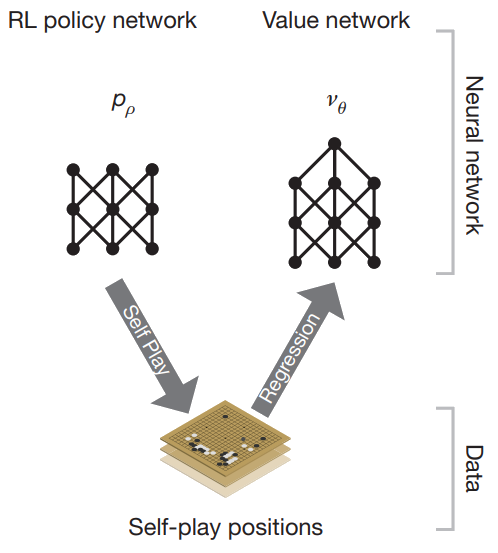
\includegraphics[width=5cm]{ressources/RL_and_VN}
	\end{center}
\end{frame}

\begin{frame}{AlphaGo}{Fast rollout policy}
	\begin{itemize}
		\item Politique de simulation rapide utilisé dans le MCTS.
		\item Entraîné avec le même modèle que le SL, mais avec une politique $p_\pi$ et une architecture beaucoup plus simple.
		\item Elle obtient des résultats moins précis mais avec une vitesse de calcul bien supérieure: précision de 24.2\% et temps d'évaluation de 2 $\mu s$ .
	\end{itemize}
\end{frame}


\begin{frame}{AlphaGo}{MCTS}

\end{frame}
